\section{Architektura mikroserwisowa}

\par Wykorzystanie architektury mikroserwisowej zapewnia wiele pozytywnych cech, takich jak: 
\begin{itemize}
    \item modularność,
    \item decentralizację,
    \item skalowalność,
    \item oraz zastępowalność i ulepszalność.
\end{itemize}
Jednak stworzenie złożonego systemu rozproszonego, wymaga odpowiedniego podziału odpowiedzialności, jak i znacząco utrudnia monitorowanie i \emph{debug}owanie.

\par Biorąc pod uwagę domenę naszego systemu jesteśmy w stanie wyodrębnić podstawowe zadania oraz oddelegować je do poszczególnych mikroserwisów. W naszym systemie występują: \emph{Message Broker}, \emph{Logger Service}, \emph{API}, \emph{HQ Service}, \emph{Decision System Service} oraz patrole.

% TODO Dopisać bazę danych, jeżeli takowa się pojawi

\par Główną odpowiedzialnością \emph{Message Broker}a w systemie jest centralizacja przesyłu informacji oraz zarządzanie nimi. W tym celu wybrano \emph{RabbitMQ}, który posiada szereg cech przemawiających na jego korzyść. Warto wymienić jego wysoką dostępność, niezawodność, skalowalność oraz elastyczność. \emph{RabbitMQ} obsługuje wiele protokołów komunikacyjnych, takich jak \texttt{AMQP}, \texttt{MQTT} i \texttt{STOMP}, co sprawia, że jest wszechstronnym narzędziem. Dodatkowo oferuje funkcje, takie jak potwierdzanie wiadomości, wzorce \emph{routing}u oraz obsługę opóźnionych wiadomości. Na podstawie badania przeprowadzonego przez \emph{CloudAMQP}\cite{CLOUDAMQP_RABBITMQ_BENCHMARK}, \emph{RabbitMQ} jest w stanie przetworzyć ponad 40 000 wiadomości na sekundę, co świadczy o jego wydajności i przydatności w ramach realizacji tego systemu. Więcej szczegółów dotyczących komunikacji między mikroserwisami można znelźć w podrozdziale \ref{sec:infrastrukturaKomunikacyjna}.

\par Głównymi obowiązkami \emph{HQ Service}u są odbieranie zgłoszeń incydentów występujących w mieście oraz zarządzanie patrolami poprzez monitorowanie ich stanów i wydawanie odpowiednich rozkazów. Ten serwis zawiera także informacje na temat obecnego stanu miasta i promuje wszystkie zdarzenia domenowe\english{Domain Event}, jako odpowiednio zmapowane wydarzenia integracyjne\english{Integration Event}, aby ogłosić zmianę stanu systemu dla pozostałych zainteresowanych serwisów. Więcej na ten temat opisane jest w podrozdziale \ref{sec:infrastrukturaKomunikacyjna}. Tutaj znajduje się \emph{HQ Agent}, odpowiedzialny za zarządzanie i komunikację z agentami patroli (\ref{sec:implementacjaAgentow}).

\par \emph{API} w tym systemie nie pełni aktywnej roli, ale działa w sposób pasywny. Jego głównym zadaniem jest obserwacja zmian i gromadzenie danych. Stanowi ono \emph{back end} dla interfejsu użytkownika, co oznacza, że działa w roli serwera, udostępniając dane dla aplikacji klienckiej. Umożliwia generowanie raportów opartych na zbieranych informacjach, które są agregowane z wydarzeń występujących w systemie. Ponadto, pozwala na prezentację obecnego stanu systemu, co jest istotne dla monitorowania i podejmowania decyzji.

\par \emph{Logger Service} ma za zadanie agregować logi z systemu, a do tego celu wykorzystuje \emph{Grafana Loki}\cite{GRAFANA_LOKI_SITE}. Jest to system do zarządzania logami, stworzony przez \emph{Grafana Labs}. Wybór tego narzędzia był podyktowany kilkoma czynnikami, w tym otwartą licencją \texttt{AGPLv3}, łatwością wdrażania w kontenerach \emph{Docker}\cite{DOCKER_SITE} oraz integracją z platformą \emph{Grafana}\cite{GRAFANA_SITE}. \emph{Grafana} zapewnia rozwiązania do monitorowania i wizualizacji danych przechowywanych w Loki. System ten wyróżnia się wysoką skalowalnością oraz prostotą w filtrowaniu otrzymywanych komunikatów, co czyni go efektywnym narzędziem do zarządzania logami w systemie.

\par Każdy patrol składa się z trzech typów mikroserwisów, które komunikują się ze sobą: \emph{Navigation Service}, \emph{Gun Service} i \emph{Patrol Service}. \emph{Patrol Service} pełni rolę punktu centralnego, który integruje pozostałe serwisy. W jego wnętrzu znajduje się agent patrolu, który zakłada funkcjonowanie w radiowozie jako komputer pokładowy.

\par \emph{Navigation Service} jest odpowiedzialny za obsługę nawigacji \emph{GPS}. Serwis ten działa na urządzeniu nawigacyjnym i jest w stanie określić obecną pozycję oraz prowadzić nawigację do wybranego punktu. W skład \emph{Navigation Service} wchodzi \emph{Navigation Agent}, który nadaje otrzymane ze środowiska informacje o obecnej pozycji.

\par Z kolei \emph{Gun Service} to prosty serwis, którego celem jest informowanie innych serwisów o wystrzałach z danego pistoletu. Za przekazywanie tej informacji dalej odpowiada \emph{Gun Agent}. Szczegółowe opisy tych agentów można znaleźć w podrozdziale \ref{sec:implementacjaAgentow}.

\par W aplikacji, ze względu na dużą współdzieloną funkcjonalność między wieloma mikroserwisami, zastosowano wydzielenie tych funkcjonalności do osobnych bibliotek. Architektura aplikacji opiera się na podziale na trzy główne warstwy: wykonawczą (nazywaną w kodzie \emph{Service}), infrastruktury\english{Infrastructure} oraz aplikacji\english{Application}. Każda z tych warstw może zawierać logikę specyficzną dla danego serwisu, ale także posiada swój odpowiednik w wersji współdzielonej\english{Shared}, w której znajdują się fragmenty kodu wykorzystywane przez wszystkie serwisy. Dla przykładu, figura \ref{fig:architectureSharedCodeExample} przedstawia diagram zależności infrastruktury znajdującej się w \emph{HQ Service} i w \emph{Patrol Service}. Dodatkowo istnieje warstwa symulacji, która zawiera implementacje serwisów komunikujących się z symulacją. Dokładniejszy opis tej warstwy znajduje się w podrozdziale \ref{sec:symulacja}.

\begin{figure}
    \centering
    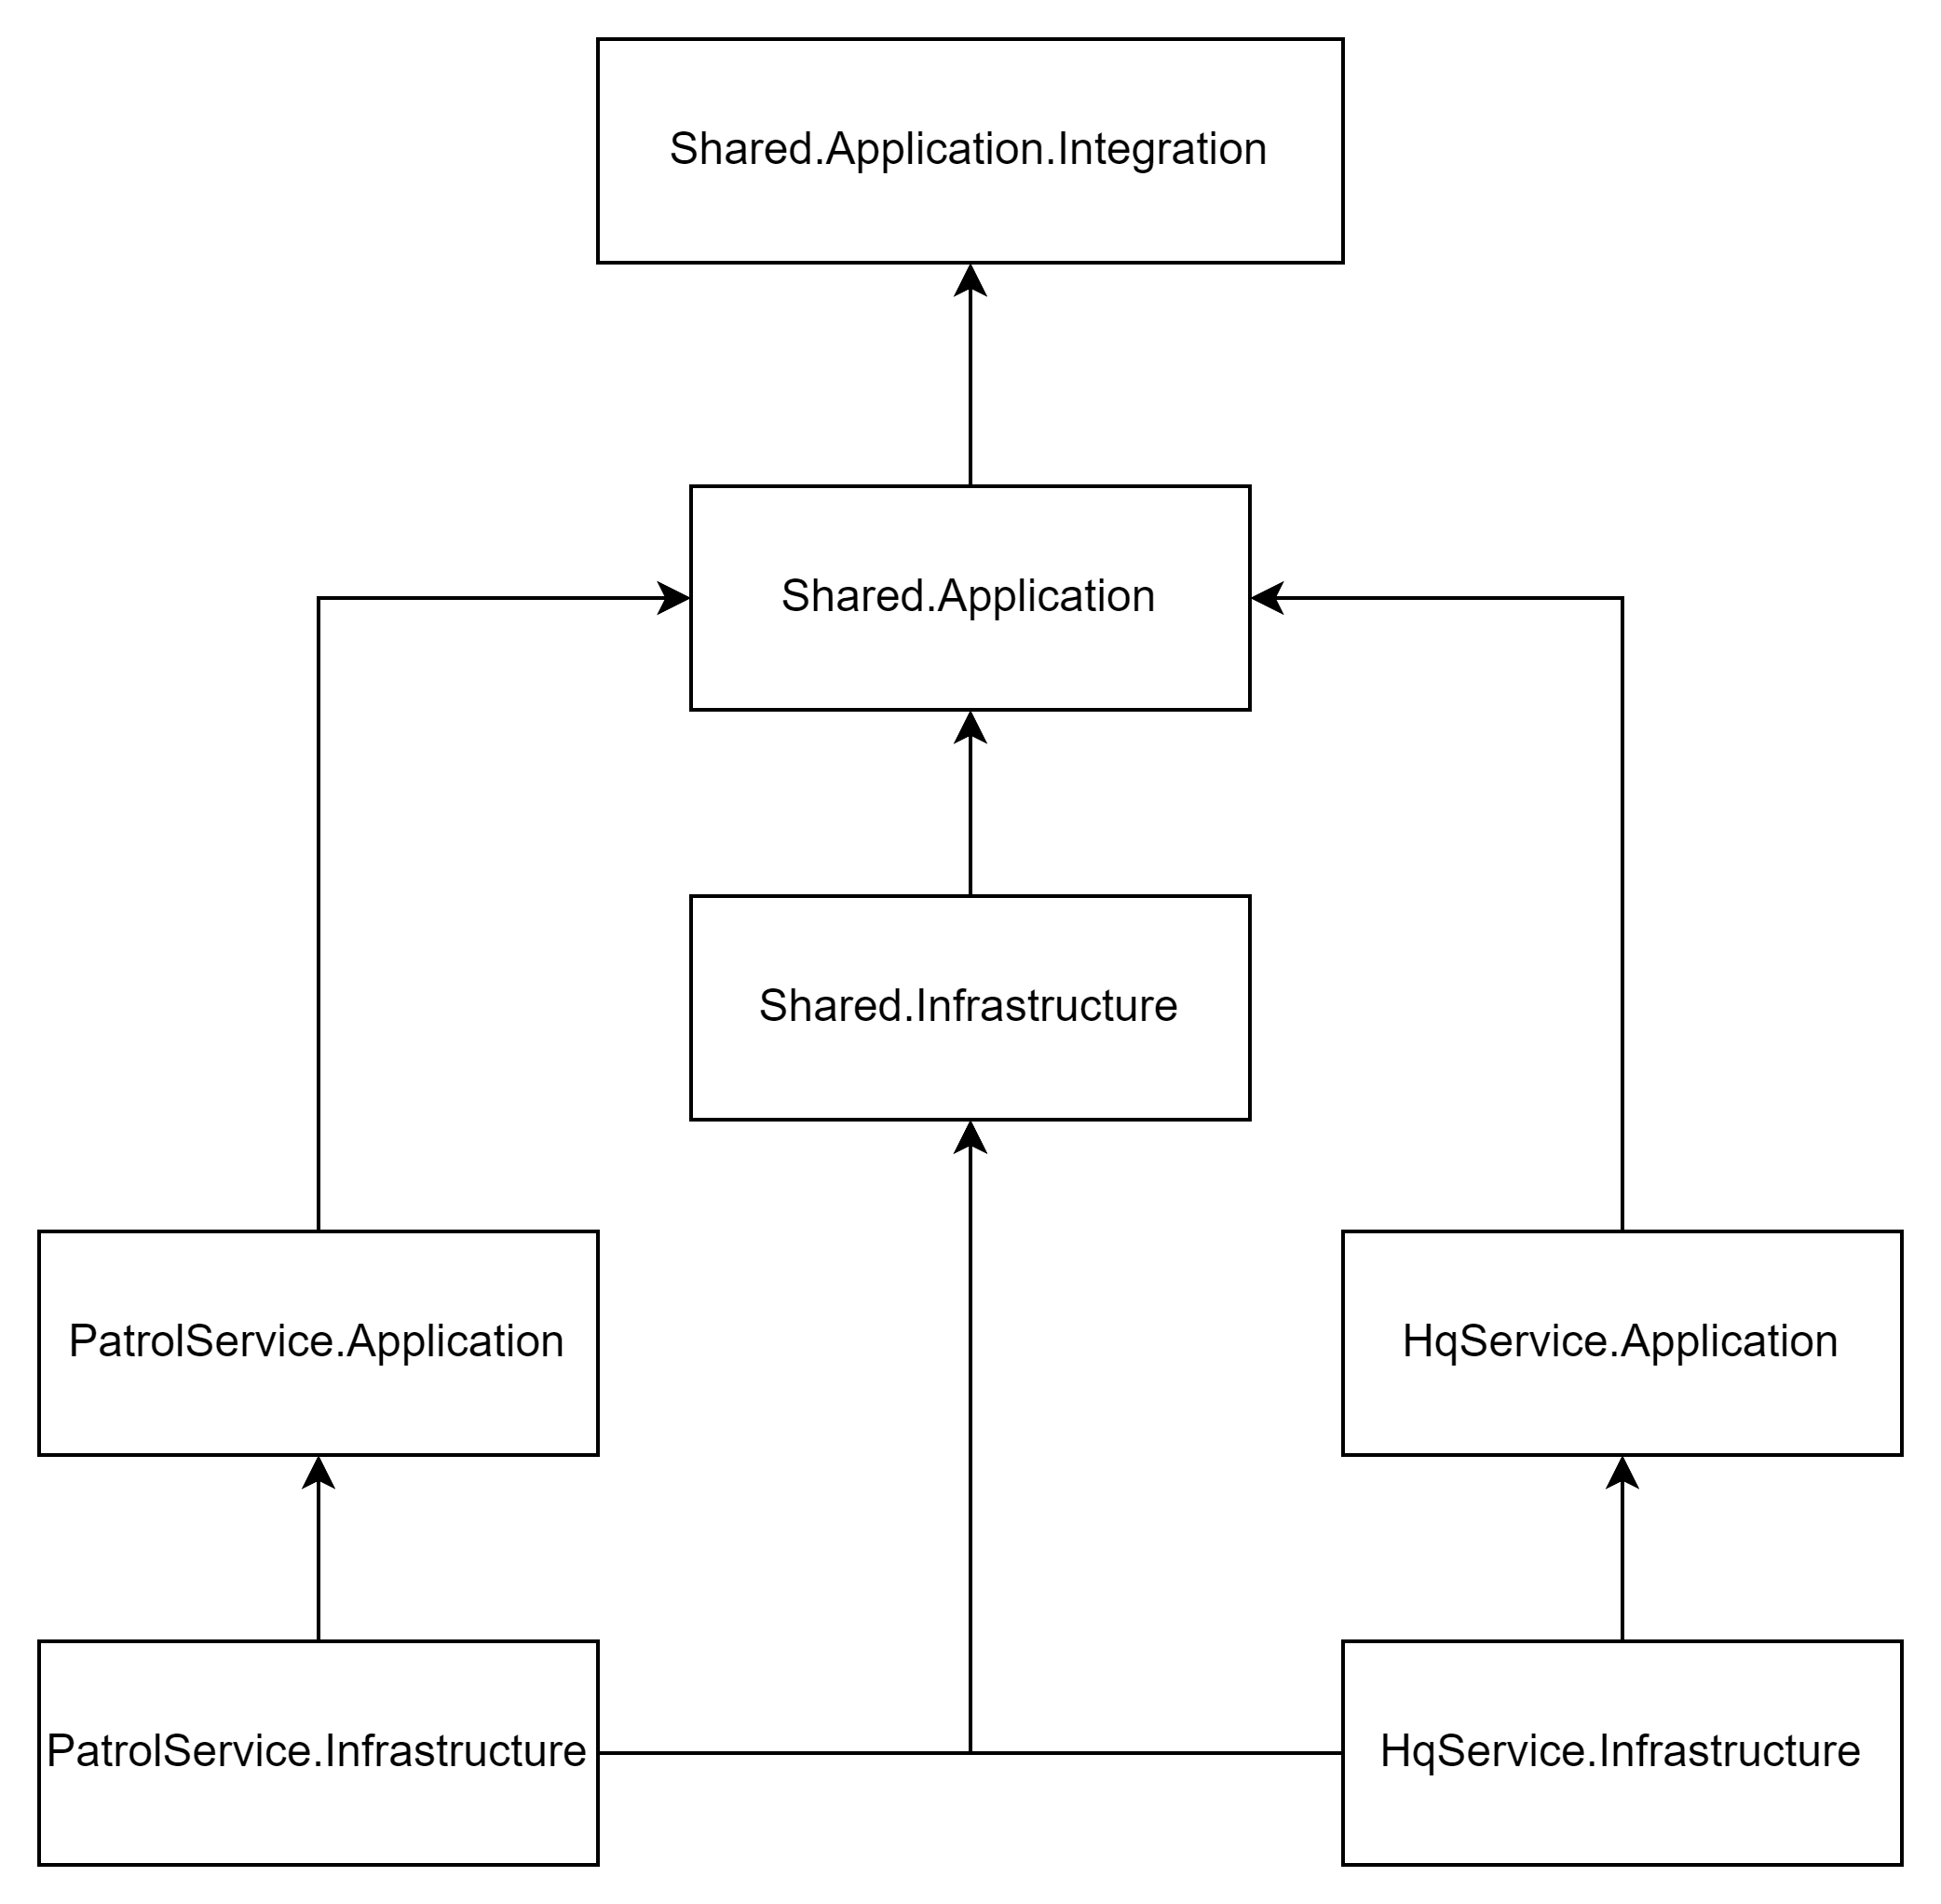
\includegraphics[width=\linewidth]{Architecture - Shared Code - Example}
    \caption{Fragment diagramu zależności przedstawiającego idee współdzielenia kodu pomiędzy serwisami}
    \label{fig:architectureSharedCodeExample}
    \source{Opracowanie Własne}
\end{figure}

\par Warstwa współdzielona zawiera także definicje obiektów domenowych\english{Domain}, bazową implementację agenta oraz wiadomości wysyłane między agentami, które są dokładniej opisane w podrozdziale \ref{sec:implementacjaAgentow}. Dodatkowo, w tej warstwie znajdują się wiadomości integracyjne, które służą do komunikacji między różnymi serwisami. Wyróżniamy trzy rodzaje wiadomości integracyjnych: zdarzenia\english{Event}, zapytania\english{Query} i komendy\english{Command}.

\par Zdarzenia mają za zadanie informować o zmianach w systemie i mogą być odbierane przez dowolną ilość odbiorców. System nie oczekuje żadnej odpowiedzi po publikacji zdarzenia.

\par Zapytania służą do pozyskiwania informacji od innego serwisu. Przewiduje się, że dane zapytanie obsłuży dokładnie jeden odbiorca, który jest wskazany w polu \texttt{Receiver}, i udzieli odpowiedzi w określonym formacie.

\par Komendy służą do wydawania poleceń innemu serwisowi. Mogą mieć tylko jednego odbiorcę, również wskazanego w polu \texttt{Receiver}, i mogą, ale nie muszą, oczekiwać na odpowiedź.

\par Detale dotyczące przesyłania tych wiadomości pomiędzy serwisami opisuje podrozdział \ref{sec:infrastrukturaKomunikacyjna}.

\par Biorąc pod uwagę wszystkie te dane rysuje się nam złożony, wielowarstwowy, ale jednocześnie bardzo modularny system. Aby lepiej zarządzać zależnościami w kodzie, zastosowana została biblioteka \emph{Autofac}\cite{AUTOFAC_SITE}. Pozwala ona na tworzenie modułów, które dodane do naszej aplikacji, samodzielnie załadują odpowiednie zależności w kodzie.

\par Rysunek \ref{fig:architectureNavigationServiceFullDiagram} przedstawia pełen diagram zależności dla \emph{Navigation Service}. Możemy w nim zaobserwować wszystkie rodzaje warstw. Te zaczynające się od \texttt{NavigationService} są specyficzne dla \emph{Navigation Service}. Warstwy znajdujące się w przestrzeni nazw \texttt{Shared}, posiadają kod wspólny dla wszystkich serwisów. Dodatkowo widoczny jest tutaj projekt \texttt{Simulation.Communication}. Zawiera on definicje wiadomości wysyłanych i odbieranych przez symulację. Więcej na ten temat znajduje się w podrozdziale \ref{sec:symulacja}. Analogicznie wyglądają zależności w pozostałych serwisach.

\begin{figure}
    \centering
    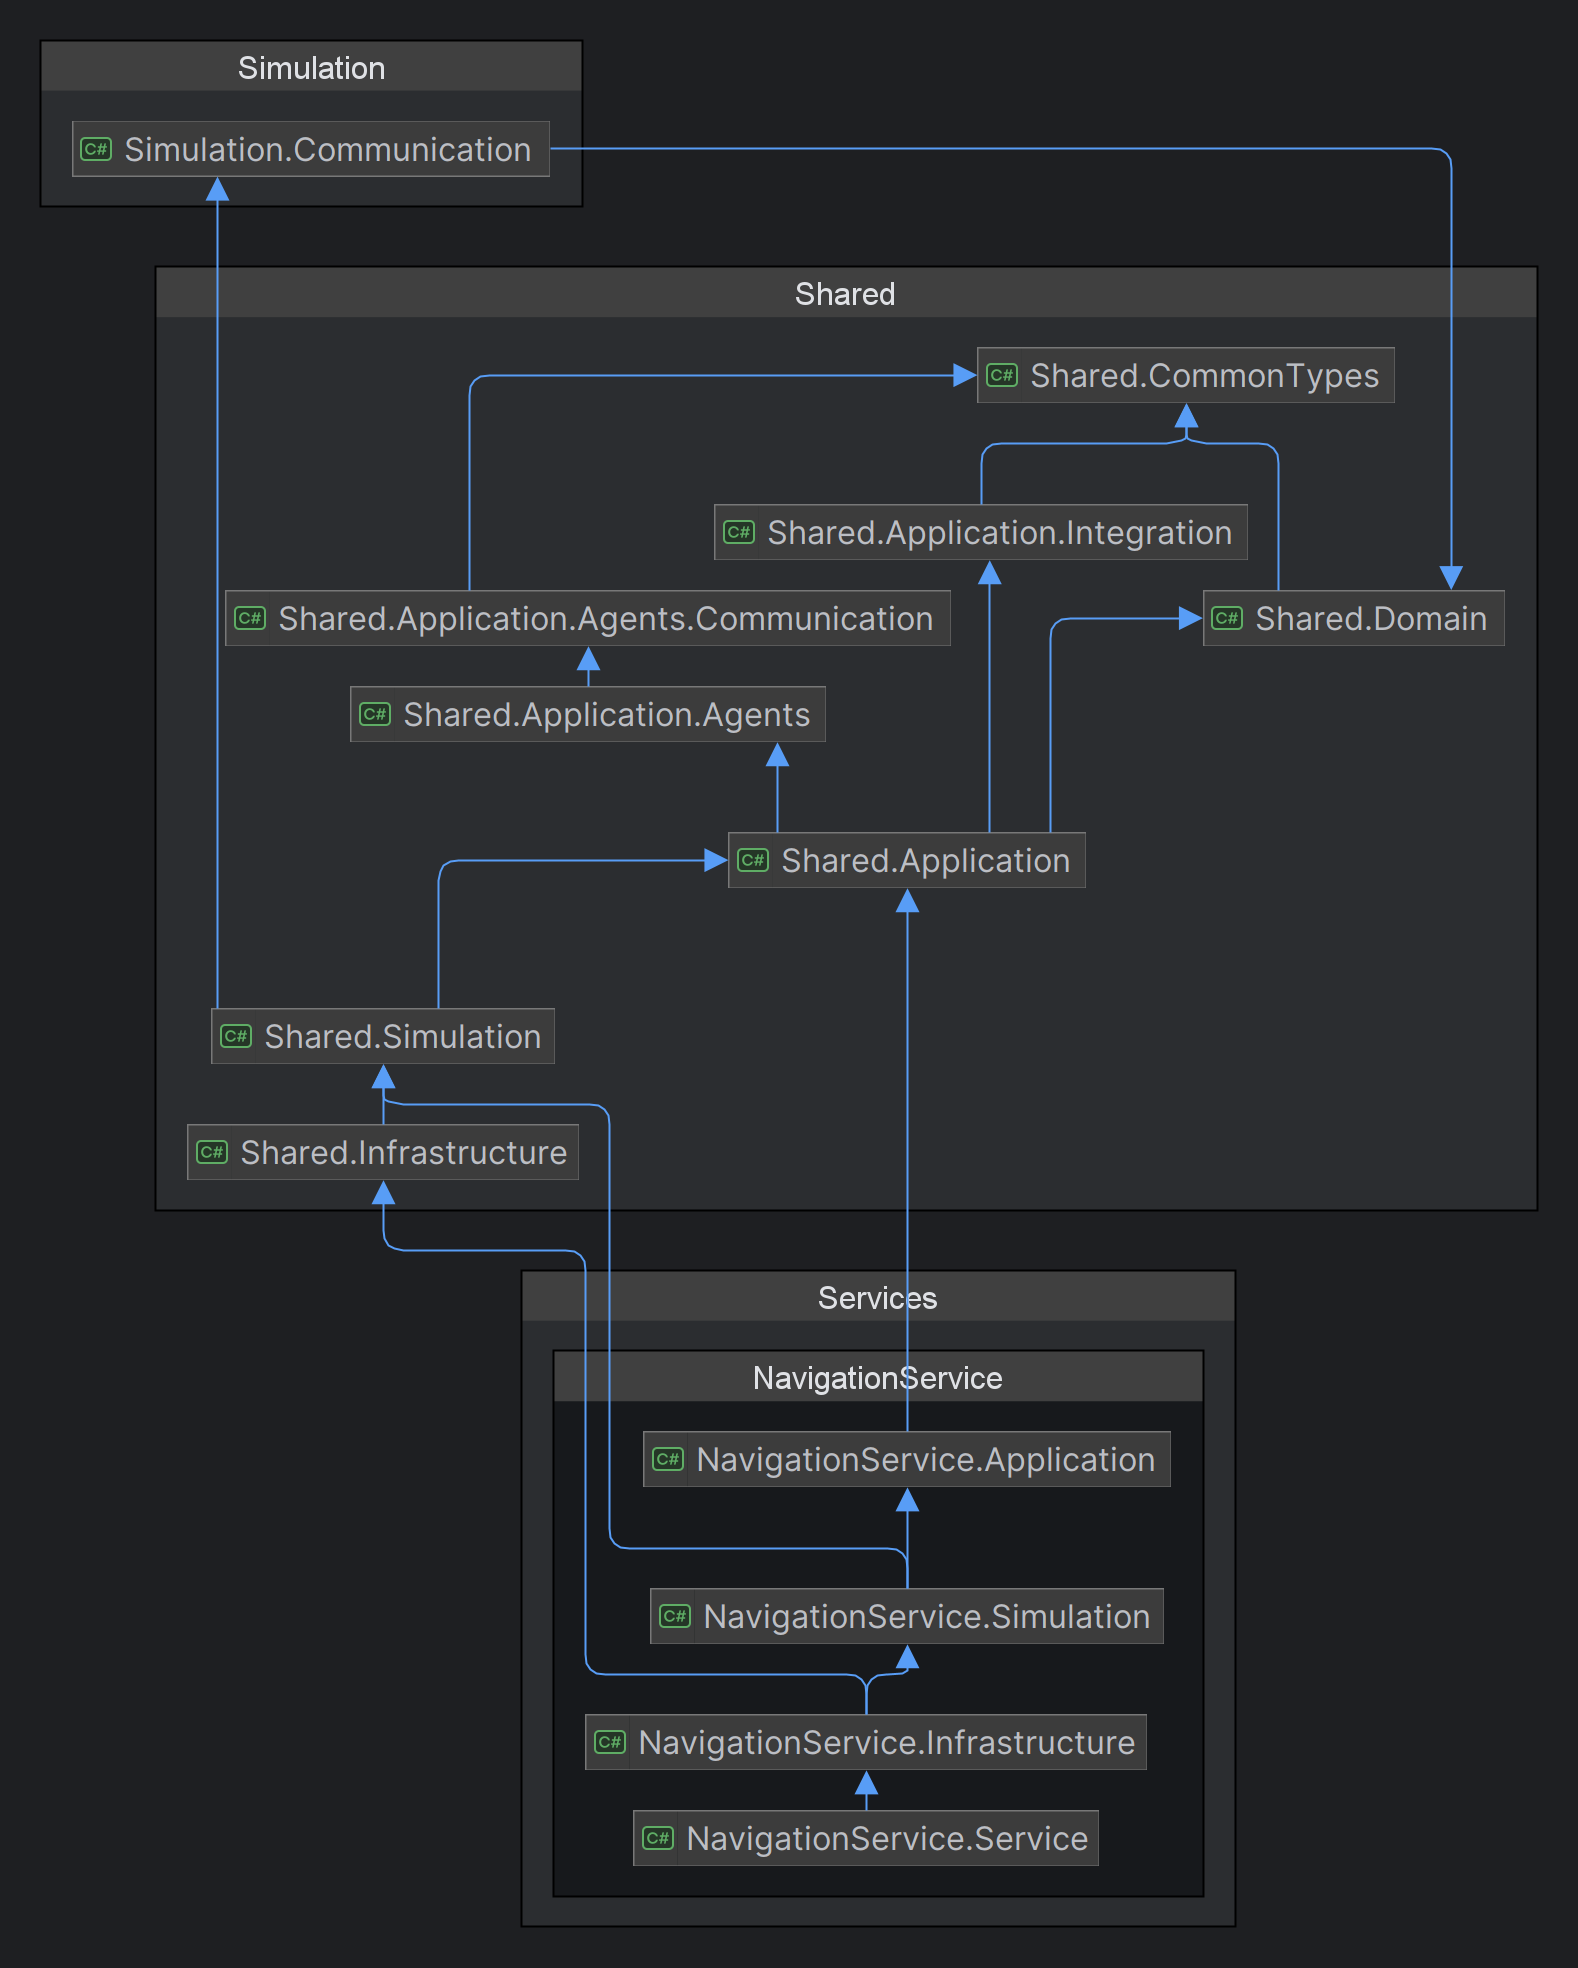
\includegraphics[width=\linewidth]{Architecture - Navigation Service - Full Diagram}
    \caption{Pełen diagram zależności dla \emph{Navigation Service}}
    \label{fig:architectureNavigationServiceFullDiagram}
    \source{Opracowanie Własne}
\end{figure}